% ----------------------------------------------
% CU STRATEGIQUE
% ----------------------------------------------
\newpage
\subsubsection{CU Échanger des trames CAN}
\paragraph{Description graphique}
\medskip
\begin{minipage}{1\linewidth}
    \centering
    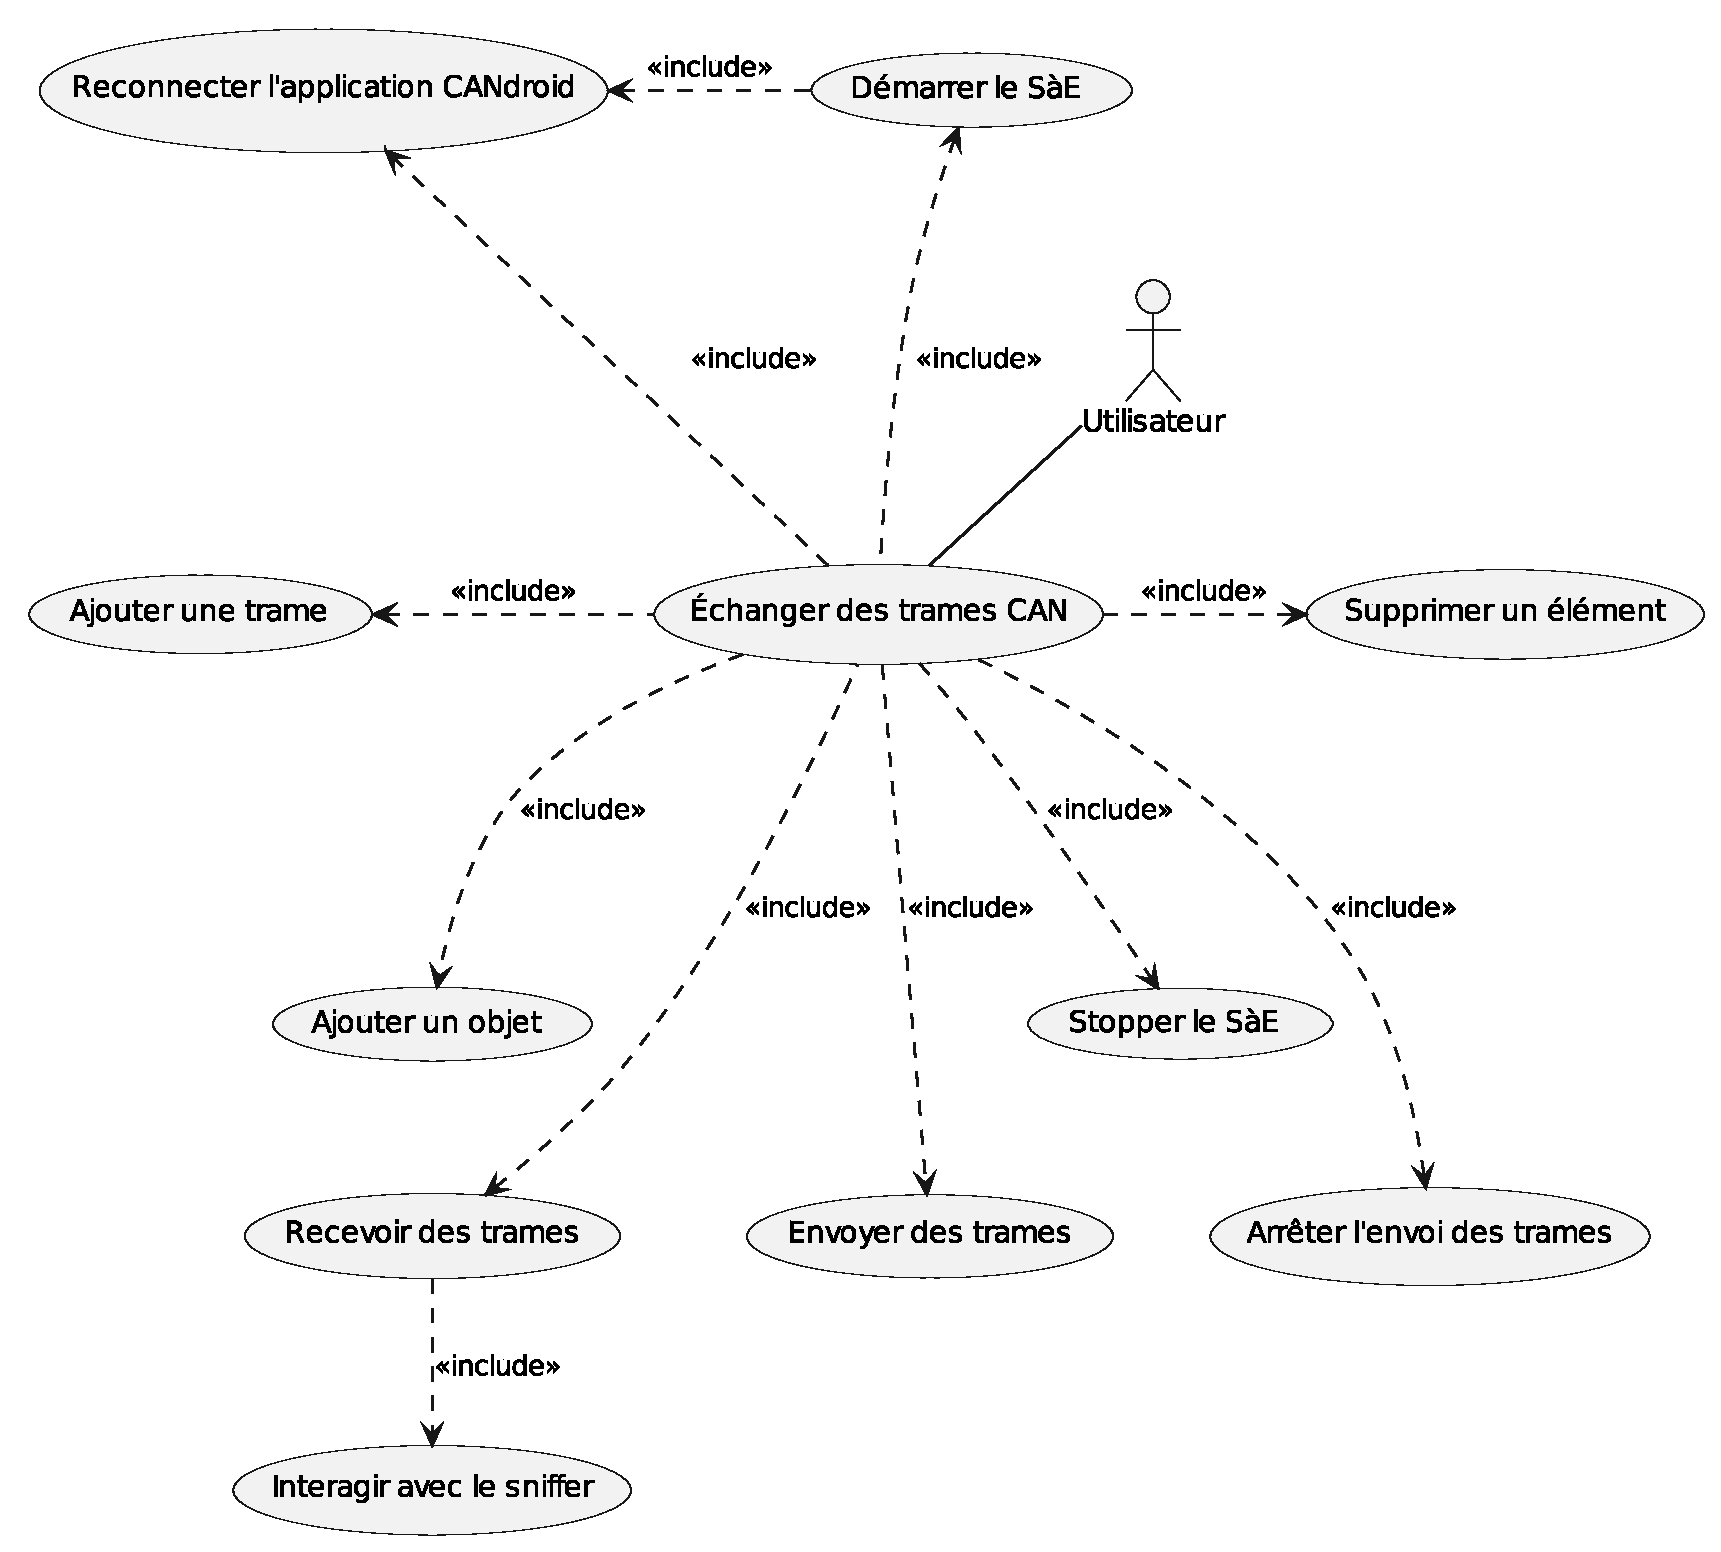
\includegraphics[width=15cm]{../../specification/schemas/cu_strat}
    \captionof{figure}{CU Échanger des trames CAN}
    \label{schema_cu_strat}
\end{minipage}

\newpage
\paragraph{Description textuelle}
\medskip

\begin{longtable}[l]{|p{3cm}|p{11.7cm}|}
    \hline
    
        Titre & Échanger des trames CAN.\\
    \hline
    
        Résumé & Utilisateur peut échanger des trames CAN avec Tableau de Bord. \\
    \hline
    
        Portée & SàE.\\
    \hline
    
        Niveau & Stratégique.\\
    \hline
    
        Acteurs directs & Utilisateur.\\
    \hline 
    
        Acteurs indirects & N.A. \\
    \hline
    
    Préconditions & 
        \begin{itemize}
            \item Tableau de Bord et la Raspberry Pi sont fonctionnels.
            \item Le programme {\nomLogiciel} est installé sur la Raspberry Pi.
            \item L'application {\nomApplication} est téléchargée sur le Smartphone.
            \item Le matériel est fonctionnel.
        \end{itemize} \\
    \hline
    
    Garanties \newline minimales & 
    \begin{itemize}
        \item L'application {\nomApplication} est utilisable.
    \end{itemize}
         \\
    \hline
    
    Garanties en cas de succès & 
    \begin{itemize}
        \item Utilisateur peut échanger des trames CAN entre Tableau de Bord et l'application {\nomApplication}.
        \item Utilisateur est capable d'observer les trames CAN reçues et d'en envoyer des nouvelles.
        \item Utilisateur est capable d'ajouter des objets ainsi que d'ajouter des trames à envoyer.
    \end{itemize}
         \\
    \hline
    
    Scénario nominal &
    \begin{enumerate}
        \item Utilisateur \underline{démarre le SàE}.
        \item Le SàE commence à \underline{recevoir des trames}.
        \item Utilisateur demande à \underline{ajouter un objet}.
        \item Utilisateur demande à \underline{ajouter une trame}.
        \item Utilisateur demande à \underline{envoyer des trames}.
        \item Le SàE diffuse les trames sur le bus CAN.
        \item Utilisateur demande à \underline{arrêter l'envoi des trames}.
        \item Utilisateur demande à \underline{supprimer un élément}.
        \item Utilisateur \underline{stoppe le SàE}.
    \end{enumerate} \\
    \hline

    Variantes & \newline
        \textbf{2,5 [La connexion n'est pas établie et Utilisateur ne souhaite pas se reconnecter]} \newline
            2,5.a.1. Va en 3. \newline
        \newline
        \textbf{2,5 [La connexion n'est pas établie \& Utilisateur souhaite se reconnecter]} \newline
            2,5.b.1. Utilisateur demande à \underline{reconnecter l'application {\nomApplication}} au programme {\nomLogiciel}. \newline
            2,5.b.2. Va en 2.\newline
        \newline
        \textbf{3,4,5,7,8 [Utilisateur souhaite stopper le SàE]}\newline
            3,4,5,7,8.a.1. Va en 9. \newline
        \newline
        \textbf{3,4,5,7,9 [Un élément existe \& Utilisateur souhaite supprimer un élément]}\newline
            3,4,5,7,9.a.1. Va en 8. \newline
        \newline
        \textbf{3,4,5,8,9 [Des trames sont en cours d'envoi \& Utilisateur souhaite arrêter l'envoi de trames]} \newline
        3,4,5,8,9.a.1. Va en 7. \newline
        \newline
        \textbf{3,4,7,8,9 [Au moins une trame existe, aucune trame n'est en cours d'envoi \& Utilisateur souhaite envoyer une trame]} \newline
        3,4,7,8,9.a.1. Va en 5. \newline
        \newline
        \textbf{3,5,7,8,9 [Utilisateur souhaite ajouter une trame \& au moins un objet existe]} \newline
        3,5,7,8,9.a.1. Va en 4. \newline
        \newline
        \textbf{4,5,7,8,9 [Utilisateur souhaite ajouter un objet]} \newline
            4,5,7,8,9.a.1. Va en 3. \newline
        \newline
        \textbf{5 [Il n'y a pas de trames à envoyer]} \newline
            5.a.1. Va en 8. \newline
        \newline
        \textbf{7 [Il n'y a pas de trames en cours d'envoi]} \newline
            7.a.1. Va en 8. \newline
        \newline
        \textbf{8 [Il n'y a pas d'éléments à supprimer]} \newline
            8.a.1. Va en 9. \newline
        \\
    \hline

    Extensions & \newline
        \textbf{2,6 [Utilisateur souhaite forcer l'arrêt du système]} \newline
        2,6.a.1. Va en 9. \newline
        \newline
        \\
    \hline
        Informations \newline complémentaires & N.A. \\
    \hline

\end{longtable}
